\section{Simulation Studies}
\label{Sec:Simulation}

We report a number of numerical simulation studies on several properties relating to 
$\tilde{\Sigma}$ and  $\Sigma_{*}$, and their eigenvalues and eigenvectors, 
on datasets with or without influential points, to illustrate the finite sample 
efficiency and robustness properties of the proposed weighted estimators. We compare 
these proposed estimators with techniques that exists in literature, specifically, 
the Sign Covariance Matrix (SCM) and Tyler's shape matrix \citep{ref:AoS87234_Tyler}.

\subsection{Efficiency of different robust estimators}

We compare the performance of $\tilde{\Sigma}$ and $\Sigma_{*}$ with that of the 
SCM and Tyler's scatter matrix. For this study, we fix the dimension $p = 4$.
We consider six elliptical distributions, 
and from every distribution draw 10000 samples each for sample sizes $n = 20, 50, 100, 
300$ and $500$. All distributions are centered at ${\bf 0}_p$, and have covariance matrix 
$\Sigma = \diag(4, 3, 2, 1)$. 

We use the concept of principal angles 
\citep{ref:LinearAlgebraApplications9281_MiaoBenIsrael} 
to find out error estimates for the 
first eigenvector of a scatter matrix. In our case, the first eigenvector is
%
\ban
\bfgamma_1 = (1, \overbrace{0, \ldots, 0}^{p - 1})^T.
\ean
%
We measure the prediction error for an eigenvector estimator (say, $\tilde\bfgamma_{1}$), 
using the smallest angle between the true and predicted vectors, i.e. 
$ \cos^{-1} | \tilde\bfgamma_{1}^T \hat\bfgamma_1 | $. A small absolute value of this 
angle means to better prediction. We repeat this 10,000 times and calculate the 
\textbf{Mean Squared Prediction Angle}:
%
\ban
MSPA(\hat \bfgamma_{1}) =
\frac{1}{10000} \sum_{m=1}^{10000} \left( \cos^{-1} 
\left|\bfgamma_1^T \tilde\bfgamma^{(m)}_{1} \right| \right)^2.
\ean
%
where $\tilde\bfgamma^{(m)}_{1}$ is the value of $\tilde\bfgamma_{1}$ in the 
$m$-th replication, $m = 1, \ldots, 10,000$. 
The finite sample efficiency of $\tilde\bfgamma_{1}$ relative to that 
from the sample covariance matrix, i.e. $\hat\bfgamma_{1}$ is obtained as:
\ban
 FSE ( \hat\bfgamma_{1}, \hat\bfgamma_{1}) = 
 \frac{ MSPA(\hat\bfgamma_{0, 1})}{MSPA(\hat\bfgamma_{1})}.
 \ean
 
 \begin{table}[t]
\begin{scriptsize}
    \begin{tabular}{c|cc|ccc|ccc}
    \hline
    4-variate $t_5$    & SCM  & Tyler & $\tilde{\Sigma}$-H & $\tilde{\Sigma}$-M & $\tilde{\Sigma}$-P & ${\Sigma}_{*}$-H & ${\Sigma}_{*}$-M & ${\Sigma}_{*}$-P \\ \hline
    $n$=20             & 1.04 & 1.02  & 1.10   & 1.07   & 1.02  & 1.09    & 1.07    & 0.98   \\
    $n$=50             & 1.08 & 1.08  & 1.16   & 1.16   & 1.13  & 1.19    & 1.19    & 1.13   \\
    $n$=100            & 1.31 & 1.31  & 1.42   & 1.38   & 1.36  & 1.46    & 1.44    & 1.36   \\
    $n$=300            & 1.46 & 1.54  & 1.81   & 1.76   & 1.95  & 1.88    & 1.88    & 1.95   \\
    $n$=500            & 1.92 & 1.93  & 2.23   & 2.03   & 2.31  & 2.35    & 2.19    & 2.39   \\ \hline
    4-variate $t_6$     & SCM  & Tyler & $\tilde{\Sigma}$-H & $\tilde{\Sigma}$-M & $\tilde{\Sigma}$-P & ${\Sigma}_{*}$-H & ${\Sigma}_{*}$-M & ${\Sigma}_{*}$-P \\ \hline
    $n$=20             & 1.00 & 1.05  & 1.03   & 1.05   & 1.00  & 1.04    & 1.04    & 0.95   \\
    $n$=50             & 1.03 & 1.01  & 1.13   & 1.12   & 1.11  & 1.19    & 1.17    & 1.10   \\
    $n$=100            & 1.08 & 1.12  & 1.25   & 1.23   & 1.27  & 1.24    & 1.25    & 1.22   \\
    $n$=300            & 1.34 & 1.36  & 1.64   & 1.52   & 1.60  & 1.67    & 1.61    & 1.68   \\
    $n$=500            & 1.26 & 1.34  & 1.55   & 1.49   & 1.60  & 1.65    & 1.61    & 1.69   \\ \hline
    4-variate $t_{10}$ & SCM  & Tyler & $\tilde{\Sigma}$-H & $\tilde{\Sigma}$-M & $\tilde{\Sigma}$-P & ${\Sigma}_{*}$-H & ${\Sigma}_{*}$-M & ${\Sigma}_{*}$-P \\ \hline
    $n$=20             & 0.90 & 0.89  & 0.95   & 0.98   & 0.98  & 0.96    & 1.01    & 0.95   \\
    $n$=50             & 0.90 & 0.91  & 1.01   & 0.98   & 0.98  & 1.03    & 1.04    & 0.99   \\
    $n$=100            & 0.87 & 0.87  & 0.93   & 0.95   & 1.01  & 0.99    & 1.01    & 1.05   \\
    $n$=300            & 0.87 & 0.87  & 1.09   & 1.09   & 1.17  & 1.14    & 1.16    & 1.23   \\
    $n$=500            & 0.88 & 0.92  & 1.10   & 1.10   & 1.23  & 1.19    & 1.22    & 1.29   \\ \hline
    4-variate $t_{15}$  & SCM  & Tyler & $\tilde{\Sigma}$-H & $\tilde{\Sigma}$-M & $\tilde{\Sigma}$-P & ${\Sigma}_{*}$-H & ${\Sigma}_{*}$-M & ${\Sigma}_{*}$-P \\ \hline
    $n$=20             & 0.92 & 0.90  & 0.94   & 0.94   & 0.96  & 0.95    & 0.97    & 0.89   \\
    $n$=50             & 0.82 & 0.83  & 0.88   & 0.91   & 0.93  & 0.88    & 0.93    & 0.93   \\
    $n$=100            & 0.84 & 0.87  & 0.92   & 0.95   & 1.00  & 0.93    & 0.96    & 1.00   \\
    $n$=300            & 0.73 & 0.75  & 0.96   & 0.99   & 1.10  & 1.00    & 1.06    & 1.12   \\
    $n$=500            & 0.73 & 0.76  & 0.95   & 0.96   & 1.06  & 0.94    & 0.97    & 1.06   \\ \hline
    4-variate $t_{25}$  & SCM  & Tyler & $\tilde{\Sigma}$-H & $\tilde{\Sigma}$-M & $\tilde{\Sigma}$-P & ${\Sigma}_{*}$-H & ${\Sigma}_{*}$-M & ${\Sigma}_{*}$-P \\ \hline
    $n$=20             & 0.89 & 0.92  & 0.92   & 0.92   & 0.90  & 0.96    & 0.95    & 0.89   \\
    $n$=50             & 0.82 & 0.84  & 0.89   & 0.90   & 0.91  & 0.93    & 0.96    & 0.92   \\
    $n$=100            & 0.77 & 0.76  & 0.90   & 0.90   & 0.96  & 0.94    & 0.98    & 1.04   \\
    $n$=300            & 0.73 & 0.77  & 0.93   & 0.91   & 0.98  & 1.00    & 0.98    & 1.03   \\
    $n$=500            & 0.67 & 0.71  & 0.83   & 0.83   & 0.96  & 0.88    & 0.90    & 1.00   \\ \hline
    4-variate Normal   & SCM  & Tyler & $\tilde{\Sigma}$-H & $\tilde{\Sigma}$-M & $\tilde{\Sigma}$-P & ${\Sigma}_{*}$-H & ${\Sigma}_{*}$-M & ${\Sigma}_{*}$-P \\ \hline
    $n$=20             & 0.82 & 0.84  & 0.87   & 0.90   & 0.91  & 0.89    & 0.93    & 0.89   \\
    $n$=50             & 0.80 & 0.81  & 0.87   & 0.88   & 0.88  & 0.88    & 0.92    & 0.88   \\
    $n$=100            & 0.68 & 0.71  & 0.80   & 0.85   & 0.91  & 0.82    & 0.86    & 0.92   \\
    $n$=300            & 0.61 & 0.63  & 0.82   & 0.85   & 0.93  & 0.86    & 0.91    & 0.96   \\
    $n$=500            & 0.60 & 0.64  & 0.77   & 0.80   & 0.90  & 0.82    & 0.86    & 0.96   \\ \hline
    \end{tabular}
\end{scriptsize}
\caption{Finite sample efficiencies of estimators of the first eigenvector based on 
several scatter matrices in dimension $p=4$. The notation
 H, M or P after $\tilde{\Sigma}$ or ${\Sigma}_{*}$ indicates the depth function 
 used for the weights: H = halfspace depth, M = Mahalanobis depth, P = projection depth.}
\label{table:FSEtable4}
\end{table}

The results from this simulation exercise are presented in Table~\ref{table:FSEtable4}.
It can be seem that  $\tilde{\Sigma}$-based estimators (columns 3-5) 
outperform SCM and Tyler's $M$-estimator of scatter. Among the 3 depth functions 
considered, projection depth gives the best results. Its finite sample performances are 
better than Tyler's and Huber's M-estimators of scatter, as well as their symmetrized 
counterparts that are much more computationally intensive (see Table 4 in 
\cite{ref:JMVA071611_Sirkiaetal}). The affine equivariant ${\Sigma}_{*}$-based estimators (columns 6-8) are even more efficient.

\subsection{Influence function comparison}

\begin{figure}[t!]
	\centering
		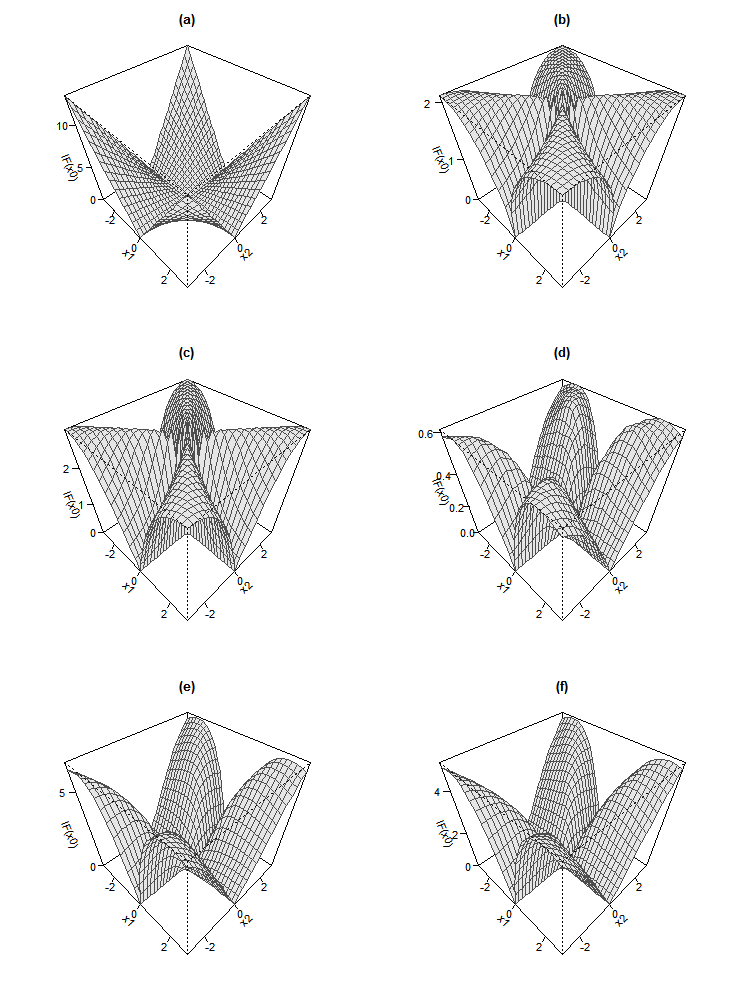
\includegraphics[width=0.8\textwidth]{./Plots/IFnorm.png}
	\caption{Plot of the norm of influence function for first eigenvector of (a) sample 
	covariance matrix, (b) SCM, (c) Tyler's scatter matrix and $\tilde{\Sigma}$ for 
	weights obtained from (d) Halfspace depth, (e) Mahalanobis depth, (f) Projection depth 
	for a bivariate normal distribution with $\bfmu = {\bf 0}, \Sigma = \diag(2,1)$}
	\label{fig:IFnorm}
\end{figure}


In Figure \ref{fig:IFnorm} we consider first eigenvectors of $\tilde{\Sigma}$, 
the Sign Covariance Matrix (SCM) 
and Tyler's shape matrix \citep{ref:AoS87234_Tyler}. We generate data from and set
$\BF \equiv \mathcal{N}_2({ 0}, \diag(2,1))$ and plot norms of the 
eigenvector influence functions for different values of $x_0$. 
Let us denote the $i$-th eigenvector of  the Sign Covariance Matrix and Tyler's shape 
matrix by  $\gamma_{S,i}$ and $\gamma_{T,i}$, respectively. 
Their influence functions are given  as follows:
%
\ban
 IF(x_0; \gamma_{S,i}, \BF) & = 
\sum_{k=1; k \neq i}^p \frac{\BS_{ik}(\Lambda^{1/2} z_0, { 0})}{\lambda_{S,i} - \lambda_{S,k}} \gamma_k; \\
%\quad 
& \text{ where }
\lambda_{S,i} = \BE_Z \left( \frac{\lambda_i z_i^2}{\sum_{j=1}^p \lambda_j z_j^2} \right),\\
IF(x_0; \gamma_{T,i}, \BF) & =  (p+2) \sum_{k=1; k \neq i}^p \frac{\sqrt{\lambda_i 
\lambda_k}}{\lambda_i - \lambda_k}\BS_{ik}(z_0; {0}) \gamma_k. 
%\label{eqn:IFeqnTyler}
\ean
%
Panels (b) and (c) in Figure~\ref{fig:IFnorm}, corresponding to  Sign Covariance Matrix 
and Tyler's shape matrix respectively, exhibit an `inlier effect', that is, 
points close to the center  having high influence,  which results in loss of efficiency. 
On the other hand, the influence function for eigenvector estimates of the 
sample covariance matrix  (panel (a)) is 
unbounded and makes the corresponding estimates non-robust. In comparison, the 
$\tilde{\Sigma}$ corresponding to weights derived from projection depth, 
half-space depth and Mahalanobis depth  have bounded influence functions {\it and} 
small values of the influence function at `deep' points.

\subsection{Efficiency of affine equivariant robust estimator}

We study the finite sample efficiency properties of $\Sigma_{*}$ 
using a simulation exercise. 
We consider 6 different elliptic distributions,  namely, the $p$-variate multivariate 
Normal distribution and the multivariate $t$ distributions corresponding to degrees 
of freedom 5, 6, 10, 15 and 25. We compute the ARE of the estimator for the 
first eigenvector using $\Sigma_{*}$, using weights based on the projection depth 
(PD) and the halfspace depth (HSD), thus this simulation is an illustration of how 
different choices of weights affect the results in the context of 
Theorem~\ref{Thm:Eigen2}.  We consider using the sample covariance 
matrix as the baseline method for this study. The ARE values are computed by
using Monte-Carlo simulation of $10^6$ samples and subsequent numerical integration.
We report the results of this exercise in Table~\ref{table:AREtable}.  
Based on these results, we notice that  $\Sigma_{*}$  is particularly efficient in lower 
dimensions for distributions with heavier tails ($t_5$ and $t_6$), while for distributions 
with lighter tails, the AREs increase with data dimension. At higher values of $p$,
note that $\Sigma_{*}$ is almost as efficient as the sample covarnace matrix even
 when the data comes from multivariate normal distribution.

\begin{table}[t]
\centering
\begin{footnotesize}
\begin{tabular}{c|cccc|cccc}
    \hline
    & \multicolumn{4}{c|}{PD} & \multicolumn{4}{c}{HSD} \\\cline{2-9}
    Distribution & $p=2$  & $p=5$  & $p=10$ & $p=20$ & $p=2$  & $p=5$  & $p=10$ & $p=20$ \\ \hline
    $t_5$           & 4.73 & 3.99 & 3.46 & 3.26 & 4.18 & 3.63 & 3.36 & 3.15 \\
    $t_6$           & 2.97 & 3.28 & 2.49 & 2.36 & 2.59 & 2.45 & 2.37 & 2.32 \\
    $t_{10}$          & 1.45 & 1.47 & 1.49 & 1.52 & 1.30 & 1.37 & 1.43 & 1.49 \\
    $t_{15}$          & 1.15 & 1.19 & 1.23 & 1.27 & 1.01 & 1.10 & 1.17 & 1.24 \\
    $t_{25}$          & 0.97 & 1.02 & 1.07 & 1.11 & 0.85 & 0.94 & 1.02 & 1.08 \\
    MVN          & 0.77 & 0.84 & 0.89 & 0.93 & 0.68 & 0.77 & 0.84 & 0.91 \\ 
    \hline
\end{tabular}
\end{footnotesize}
\caption{Table of AREs of the estimator for the first eigenvector estimation using 
$\Sigma_{*}$, relative to using the sample covariance matrix, for different choices of 
dimension $p$. The data-generating distributions are the multivariate Normal (MVN), 
and multivariate $t$-distributions with degrees of freedom 5, 6, 10, 15 and 25. Weights 
for $\Sigma_{*}$ are based on either the projection depth (PD) or the half-space 
depth (HSD).}
\label{table:AREtable}
\end{table}

%\end{comment}



\subsection{Robust sufficient dimension reduction and supervised learning}

One of the main usages of obtaining dispersion estimators and their eigenvalues and 
eigenvectors is in \textit{dimension reduction} techniques. Examples of such uses are in 
\textit{principal component regression, partial least squares} and \textit{envelope 
methods}. We illustrate below the latter technique, in the context of 
\textit{sufficient dimension reduction} (SDR). For details on envelope methods and other 
uses of robust estimators of dispersion and eigen-structures, see 
\citet{ref:Sinica10927_Cooketal, ref:PhilTransRoyalSoc094385_AdragniCook, 
ref:JASA15599_CookZhang} 
and references and citations of these 
articles. In the context of multivariate-response ($Y_{i} \in \BR^{q}$) linear regression, 
the envelope method proposes the model $Y_{i} = \alpha + \Gamma_{1} \eta x_{i} + e_{i}$, 
where $e_{i}$ are independent mean zero Gaussian  noise terms with covariance matrix 
$\Sigma$ whose spectral representation can be written as 
\ban 
\Sigma = \Gamma \Lambda \Gamma^{T}
& = 
\left( \begin{array}{ll}
\Gamma_{0} & \Gamma_{1} 
\end{array}
\right)
\left( \begin{array}{ll}
\Lambda_{0} & 0 \\
0 & \Lambda_{1} 
\end{array}
\right)
\left( \begin{array}{l}
\Gamma_{0} \\
\Gamma_{1} 
\end{array}
\right) \\
& = \Gamma_{0} \Lambda_{0} \Gamma_{0}^{T}
+ \Gamma_{1} \Lambda_{1} \Gamma_{1}^{T}.
\ean
Thus, the eigenvectors of $\Sigma$ are partitioned into two blocks:  
$\Gamma_{1} \in \BR^{q} \times \BR^{d}$ and 
$\Gamma_{0} \in \BR^{q} \times \BR^{q-d}$, and 
the regression coefficient of $Y_{i}$ on $x_{i}$  is given by 
$\Gamma_{1} \eta$ for some $\eta \in \BR^{d} \times \BR^{p}$. 
Dimension reduction is achieved  when $d \ll p$, typically without extraneous 
assumptions like sparsity. The envelope model for generalized linear models is 
discussed in \citet{ref:PhilTransRoyalSoc094385_AdragniCook}, 
and may be used for supervised 
learning. Nonlinear regression models may also be handled similarly.

Given a set of examples $\{ (Y_{i}, X_{i}), i = 1, \ldots, n \}$, an envelope-based 
prediction for the response $Y$ for any $X$ may be obtained from 
\ban
\hat{Y} (X) & = \bigl[ \sum_{i = 1}^{n} w_{i} \bigr]^{-1}
\sum_{i = 1}^{n} w_{i} Y_{i}, 
\text{ where } \\ 
 w_{i} &= \exp \left[ -\frac{1}{\hat\sigma^2}  | \hat\Gamma_{1}^T (X - X_i) |^2 \right].
\ean
The above assumes that the covariates come from the Gaussian distribution 
$N_{p} ({\bf 0}_{p}, \sigma^{2} \BI_{p})$, and appropriate 
changes may be made for other distributions. 

We design a robust version of the above, by using weighted spatial medians for location 
parameters corresponding to the distributions of $X$ and $X | Y$, and using the first $d$ 
eigenvectors of $\tilde{\Sigma}$ as $\hat\Gamma_{1}$. A robust location estimator for 
the distribution of $X | Y$ is required for the estimation of $\sigma^2$. 
Details are available in \cite{ref:PhilTransRoyalSoc094385_AdragniCook}.
%
\begin{figure}[t!]
\begin{center}
\begin{tabular}{ll}
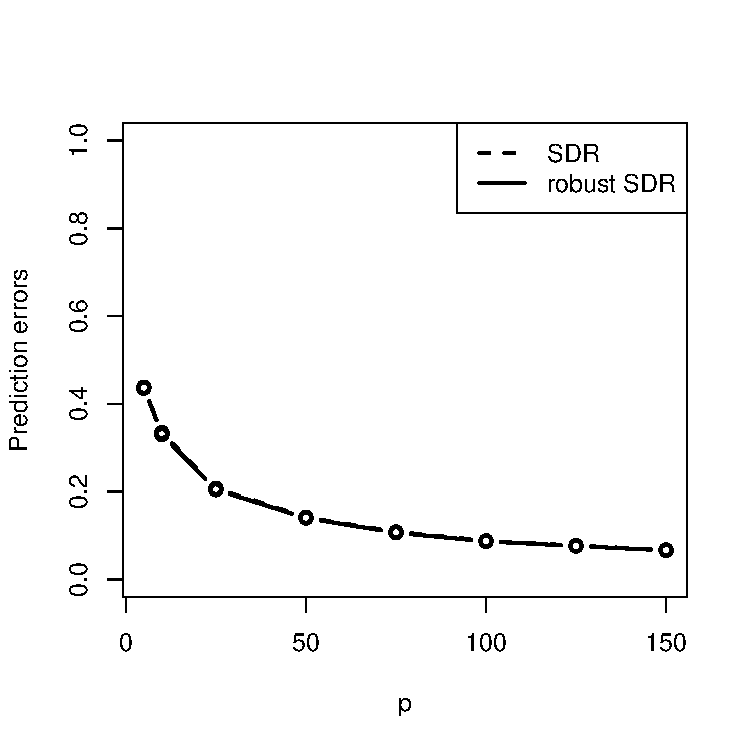
\includegraphics[width=0.4\textwidth]{./Plots/SDRcomparison_noout} &
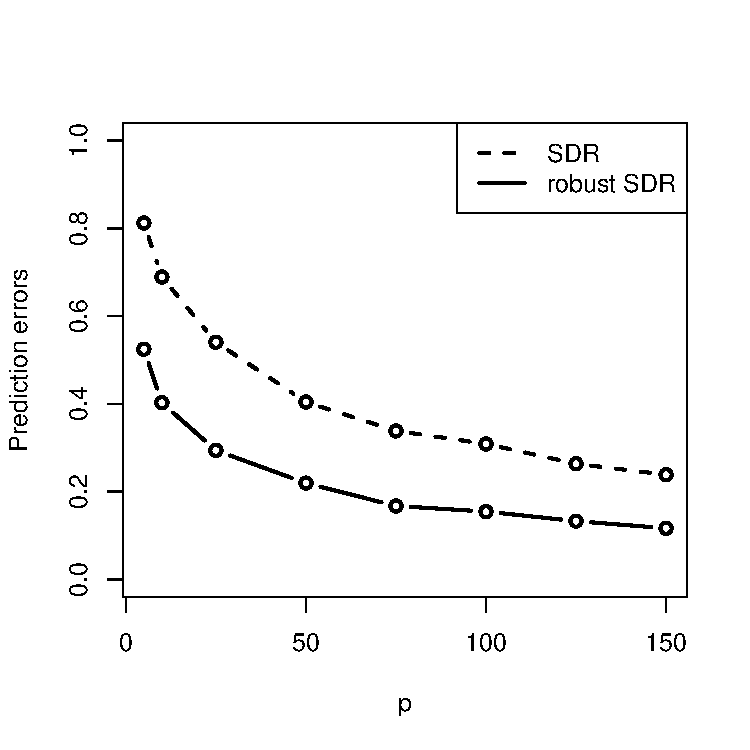
\includegraphics[width=0.4\textwidth]{./Plots/SDRcomparison_out}
\end{tabular}
\caption{Average prediction errors for two methods of SDR (a) in absence and (b) in presence of outliers}
\label{fig:SDRfig}
\end{center}
\end{figure}
%
In a non-linear regression model, we compare the performance of the robust version of 
SDR with the original method of 
\cite{ref:PhilTransRoyalSoc094385_AdragniCook} 
with or without the presence of bad leverage points in $\Sigma$. 
For any given choice of covariate dimension $p$, we take $n=200$ and $d=1$, 
and generate the responses 
$Y_1, \ldots, Y_n$ as independent standard normal, and 
$X | Y$ as Normal with mean $Y + Y^{2} + Y^3$ in each of the $p$ coordinates, 
and variance $25 \BI_p$.
We measure performances of the SDR models by their mean squared prediction error on 
another set of 200 observations  generated similarly, and taking the average of these 
errors on 100 such training-test pairs of datasets. The above steps 
are repeated for the choices of $p = 5, 10, 25, 50, 75, 100, 125, 150$.

Panel (a) of figure \ref{fig:SDRfig} compares prediction errors using both robust and 
maximum likelihood SDR estimates when the covariates contain no outliers: here the two 
methods are virtually indistinguishable. We then introduce outliers in each of the 100 
datasets by adding 100 to first $p/5$ coordinates of the first 10 observed covariate 
values, and repeat the analysis. Panel (b) of the figure shows that the robust SDR method 
remains more accurate in predicting out of sample observations for all values of $p$ than 
the standard SDR.



